%-------------------------------------------------------------------
\chapter{Introduction}
\label{ch:intro}
%-------------------------------------------------------------------
%
\begin{figure}
    \centering
    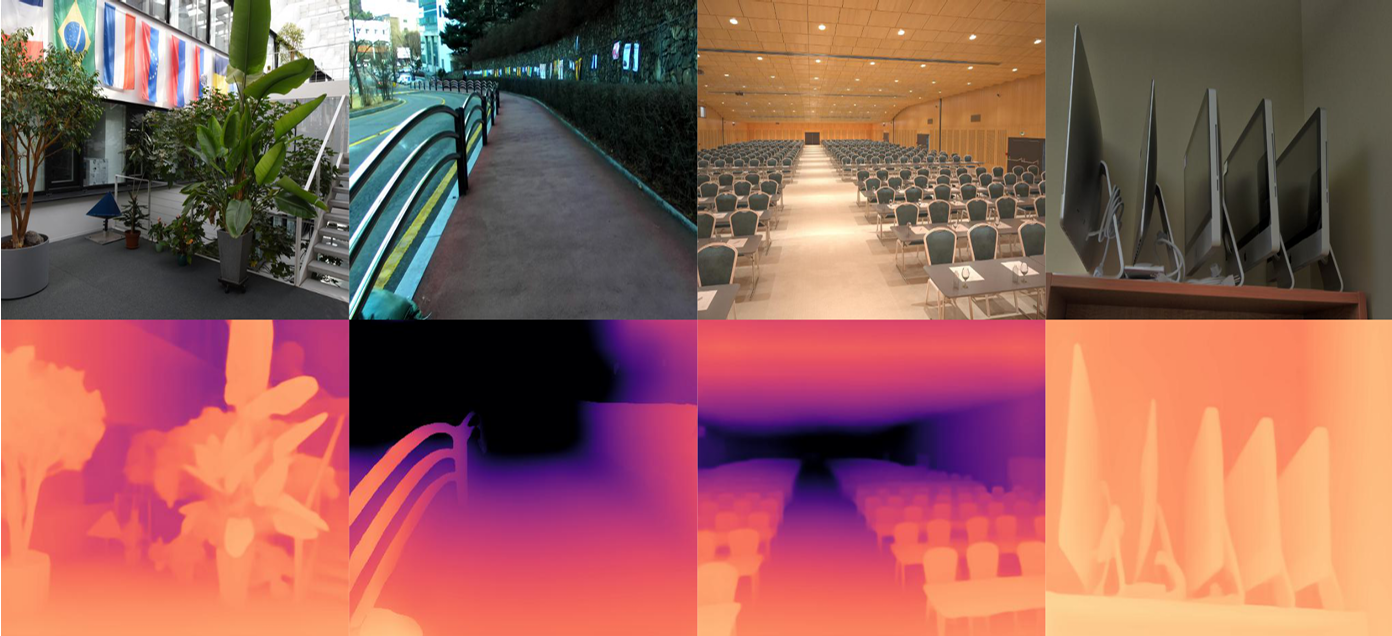
\includegraphics[scale=0.3]{figs/depth_maps_example2}
    \caption[Example of depth maps.]{
        An example of images (top) and their depth maps (bottom).
        Depth values are color-coded: darker colors correspond to farther points in space.
        Figure taken from \cite{ZoeDepth}.
        \label{fig:depth_maps_example}
    }
\end{figure}
The setting of this thesis is Single Image Depth Estimation (SIDE), also called Monocular Depth Estimation (MDE), which refers to a depth estimation problem based on only one image of the scene (Figure \ref{fig:depth_maps_example}).
Traditionally, this is done by assigning to each image pixel a depth value corresponding to the depth of the object that forms that pixel in the camera coordinate system (Figure \ref{fig:coordinates}).
Single Image Depth Estimation (SIDE) saw a growing research interest in the last years.
Its popularity is to be attributed to advancements in robotics and autonomous driving which could benefit from solving this task.
In fact, depth sensors are expensive and not reliable in various scenarios (for instance in presence of reflective surfaces).
Stereo rigs are instead difficult to use since constant calibration is required.
Hence, if depth could be accurately estimated by using only a single RGB camera, research in autonomous navigation of real-world environments would be boosted.

Deep learning is currently the leading methodology for tackling SIDE and is based on training large models on various datasets to achieve zero-shot performances, meaning to generalize on unseen datasets.
Within deep learning, the most common model is based on Convolutional Neural Networks (CNN) using an encoder-decoder architecture that works at multiple scales (Figure \ref{fig:flow_net}).
In recent years, other architectures gained popularity, in particular transformer-based architectures~\cite{denseViT, PatchFusion}, diffusion models~\cite{Marigold}, and Large Vision models (LVMs)~\cite{Marigold}.
However, in applications such as robotics and autonomous driving, large neural networks present various problems.
For instance, performing real-time inference on edge devices could be prohibitive.
Most importantly, deep learning models are well known to be black-boxes.
Their functioning is not understood by humans (it is said to be opaque) and can represent a problem in a critical application like autonomous driving, where decisions need to be explainable.
To tackle the problem of explaining deep learning models, Explainable Artificial Intelligence (XAI) approaches have been investigated in the literature~\cite{XAI_review}.
However, despite the popularity of XAI in the research community, only few works address the problem of explainability in SIDE~\cite{Hu, Dijk, towards_interpretable}.

\begin{figure}
    \centering
    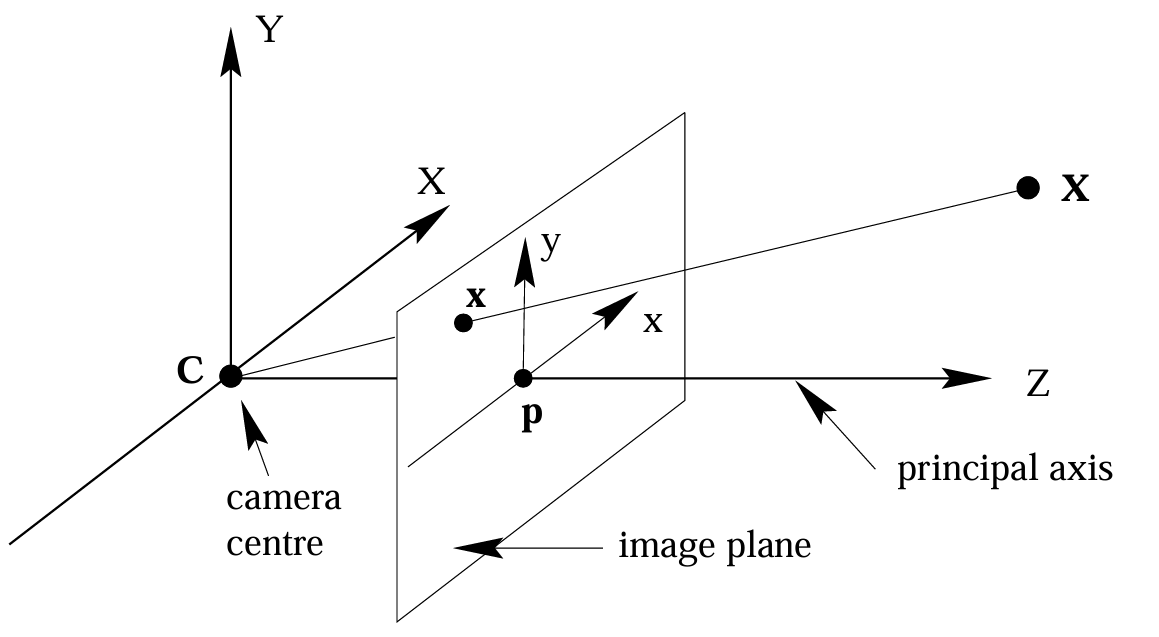
\includegraphics[scale=0.3]{figs/coordinates}
    \caption[Camera geometry.]{
        Camera geometry, image from \cite{multiview}.
        To the pixel $\mathbf{x}$ is associated the $Z$ coordinate of the point $\mathbf{X}$.
        The point $\mathbf{p}$ is called the \textit{principal point} of the camera, it will appear in chapter \ref{ch:methods}.
        \label{fig:coordinates}
    }
\end{figure}

The objective of this thesis is to investigate the concept of interpretability, central to XAI, and its relation to SIDE.
It is shown that some XAI research methods are biased and that there exist theoretical limitations to explainability that have consequences on this whole field of research.
Such limitations stem from the inability of mathematical language to capture human related concepts like the one of "explanation", this fact is referred to as explanatory gap (EG) throughout the thesis.
It is argued that since SIDE involves aspects of human cognition, it is affected by the EG as well.
Solving the SIDE task implies a minimum degree of opaqueness in the resulting method.
This makes the use of non-interpretable components necessary for solving the depth estimation task.
To reduce the impact of black-box methods on the overall interpretability of a SIDE pipeline, such methods must be confined to sub-tasks, leaving space for interpretable components.
The responsibility of the final prediction is shared between non-interpretable and interpretable components.
To further transfer responsibilities to the latter, the learning problem solved by the former has to be simplified.
Experiments are then performed to test this approach applied to patch-wise depth estimation.
The simplification of the learning problem is performed by carefully choosing the training patches, pre-processing them and using a different training loss and evaluation metrics.
Results suggest that the practice of simplifying the learning problem can be beneficial since the model scores better metrics on the simplified learning problem.

\begin{figure}
    \begin{adjustwidth}{-0.2\textwidth}{-0.2\textwidth}
    \centering
    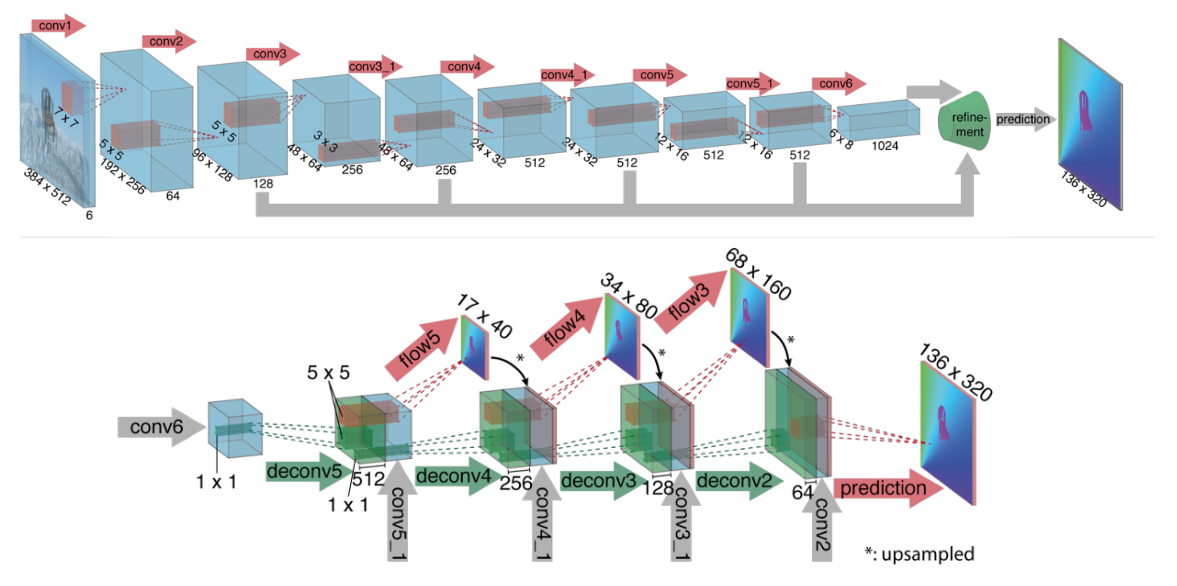
\includegraphics[scale=0.4]{figs/flow_net}
    \end{adjustwidth}
    \caption[Example of architecture used for depth estimation.]{
        FlowNet architecture from \cite{FlowNet}.
        At the top row the encoder is detailed, while the multi-scale decoder is shown at the bottom.
        This architecture was first used for optical flow estimation and later adapted to depth estimation (starting from \cite{DispNet}).
        \label{fig:flow_net}    
    }
\end{figure}

The rest of the thesis is organized as follows:
\begin{itemize}
    \item{
        Chapter \ref{ch:sota} reviews various methods for SIDE.
        Treated methods span from early days of the field to most recent developments.
        The last two sections are about XAI and influential works on interpretability of SIDE models are presented.
    }
    \item{
        Chapter \ref{ch:methods} addresses the problem of interpretability from a theoretical point of view.
        The above claims about interpretability are supported in sections \ref{sec:limits of XAI}, \ref{sec:limits of interpretability} and \ref{sec:interpretability of depth estimation}.
        In section \ref{sec:hybrid}, the formal theory of learning is quickly reviewed and possible simplifications to the problem of patch-wise depth estimation are presented and motivated.
        The last section \ref{sec:depth_fusion} proposes a design for an interpretable algorithm that stitches together the partial patch predictions.
    }
    \item{
        Chapter \ref{ch:results} presents and comments the experimental results obtained with the simplifications discussed in section \ref{sec:hybrid}.
    }
    \item{
        Chapter \ref{ch:conc} closes this thesis by summing up its contributions and suggestions for future work.
    }
\end{itemize}
%This thesis is in the field of computer vision, specifically single image depth estimation.
%Under the name of "Depth Estimation" (DE) a lot of techniques appear, but there is no formal definition that considers them all.
%DE could be defined as the study of algorithms that process one or more images of a scene and output information about its geometry.
%There exist many approaches to do this as well as many problem settings.
%The setting of this thesis is \textit{Single Image Depth Estimation} (SIDE), also called \textit{Monocular Depth Estimation} (MDE).
%It refers to a depth estimation problem based on only one image of the scene.
%As of today, this is done by assigning to each image pixel a depth value corresponding to the depth of the object that forms that pixel in the camera coordinate system, see figure~\ref{fig:coordinates} for an illustration.
%
%Images are represented as numerical tensors and the depth values corresponding to each pixel are organized in tensors as well, called depth maps.
%The mapping from an image to a depth map can be realized by some parametrized function, in deep learning these are called neural networks.
%Datasets gather examples of desired input-output pairs realizing this mapping and, thanks to a training procedure, this information can be used for tuning said parameters.
%This constitutes the essence of statistical learning problems~\cite{ML_book}.
%In figure~\ref{fig:depth_maps_example} some depth maps are depicted.
%\begin{figure}
%    \centering
%    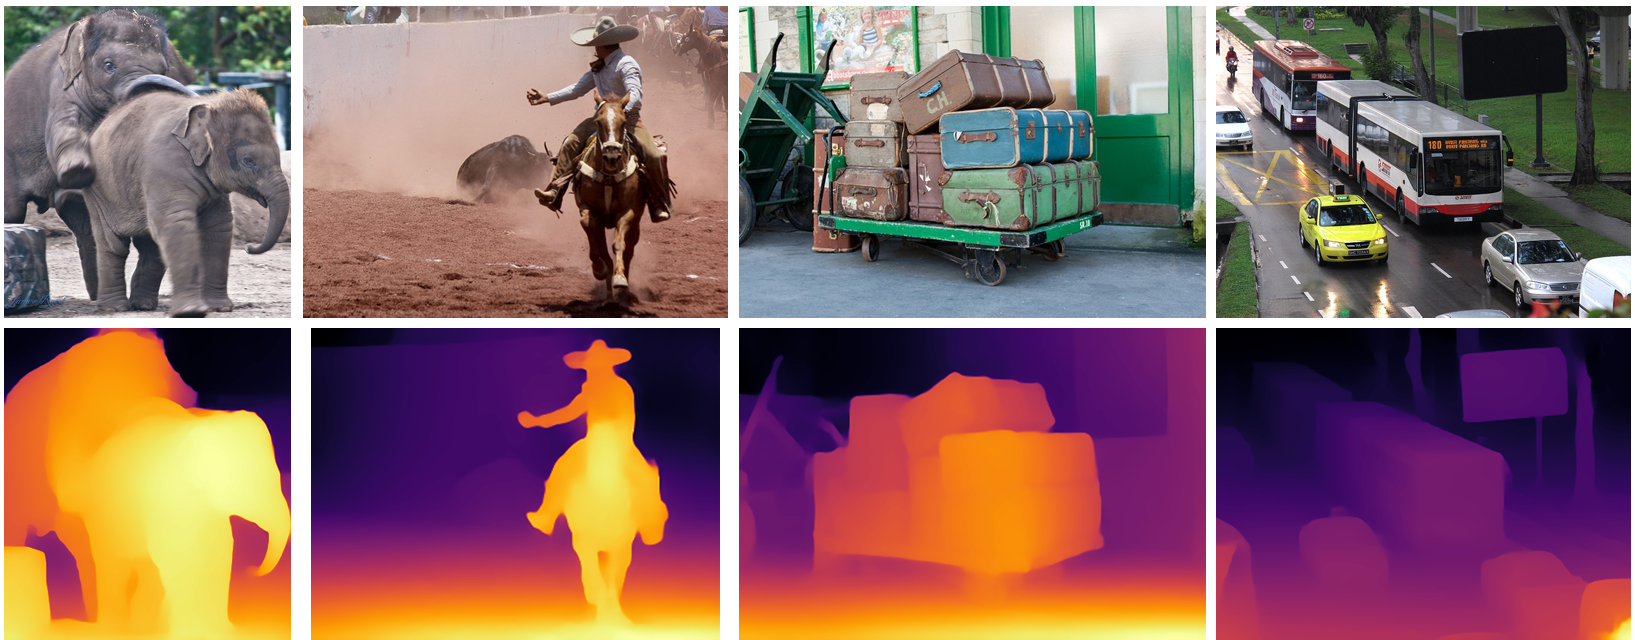
\includegraphics[scale=0.3]{figs/depth_maps_example}
%    \caption{
%        An example of images (top) and their depth maps (bottom).
%        Depth values are color-coded: darker colors correspond to farther points in space.
%        Figure taken from \cite{MiDas}.
%        \label{fig:depth_maps_example}
%    }
%\end{figure}
%
%Datasets are created by acquiring images and depth information of the scene simultaneously through the use of depth sensors~\cite{KITTI, NYUv2}.
%An alternative is to let humans annotate images~\cite{DIW}, but a different kind of depth information is collected in this way.
%In fact, depth values can be \textit{metric} or \textit{relative}.
%Metric depth values represent physical distances in some unit of measure (e.g. meters) and are the ones measured by sensors.
%Relative depth values are used only for comparing depths across the image.
%Relative depth estimation is a simpler problem than metric depth estimation and humans are able to perform it in simple settings (e.g. a human is asked to tell which pixel is closer to the camera given another).
%In the SIDE case, metric depth estimation is impossible if information about the camera acquiring the image is not available.
%Hence, SIDE is often framed as a relative depth estimation problem.
%\begin{figure}
%    \centering
%    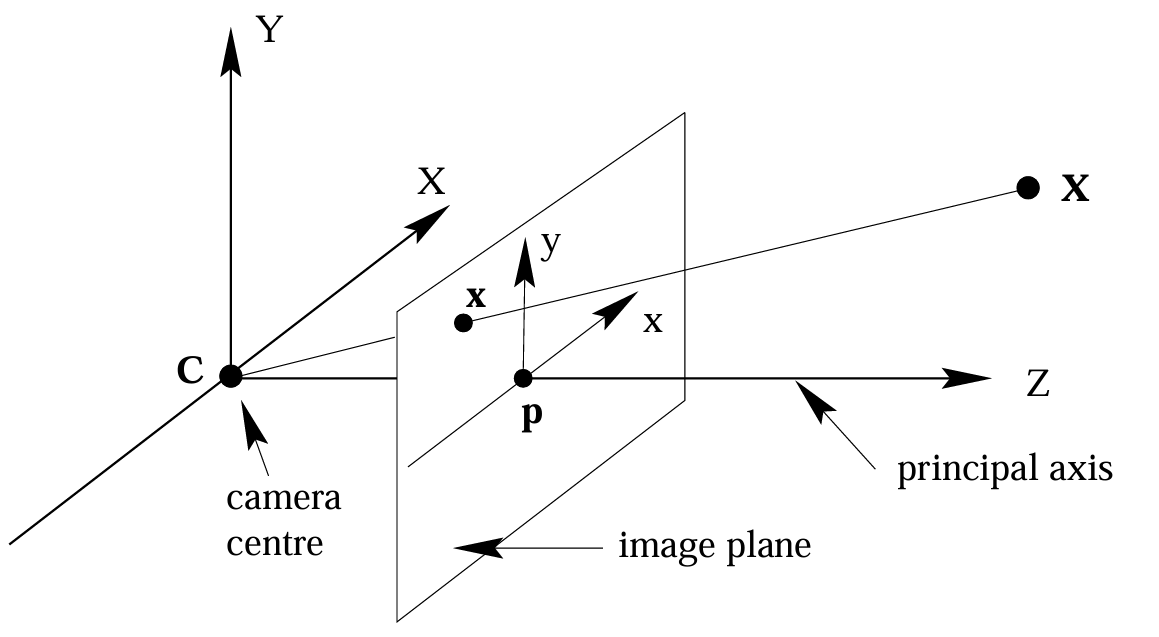
\includegraphics[scale=0.3]{figs/coordinates}
%    \caption{
%        Camera geometry, image from \cite{multiview}.
%        To the pixel $\mathbf{x}$ is associated the $Z$ coordinate of the point $\mathbf{X}$.
%        The point $\mathbf{p}$ is called the \textit{principal point} of the camera, it will appear in chapter \ref{ch:methods}.
%        \label{fig:coordinates}
%    }
%\end{figure}
%
%Two images taken from different view-angles can be used for partially reconstructing depth using epipolar geometry~\cite{multiview}.
%This fact is used in binocular depth estimation models, but it can also be used for inferring the ground truth depth map when it is unknown.
%The self-supervised learning approach to SIDE is based on these ideas, it is less effective but it does not require expensive annotated data \cite{monocular_SSL}.
%
%Single Image Depth Estimation (SIDE) saw a growing research interest in the last years.
%Its popularity is to be attributed to advancements in robotics and autonomous driving which could benefit from solving this task.
%In fact, depth sensors are expensive and not reliable in various scenarios (for instance in presence of reflective surfaces).
%Stereo rigs are instead difficult to use since constant calibration is required.
%Hence, if depth could be accurately estimated by using only a single RGB camera, research in autonomous navigation of real-world environments would be boosted.
%
%Deep learning is the leading methodology for tackling SIDE.
%The research trend is to train large models on various datasets to achieve zero-shot performances, meaning to generalize on unseen datasets.
%MiDas~\cite{MiDas} was the leading work in this direction that managed to train a model on heterogeneous datasets.
%It was done by converting each ground truth data to a common representation, in particular the authors chose to work in the disparity space.
%The most common architecture is an encoder-decoder model that works at multiple scales.
%The encoder is a classification backbone and the decoder estimates successive finer depth maps from the computed features of the encoder.
%An example of such an architecture is illustrated in figure \ref{fig:flow_net}.
%\begin{figure}
%    \begin{adjustwidth}{-0.2\textwidth}{-0.2\textwidth}
%    \centering
%    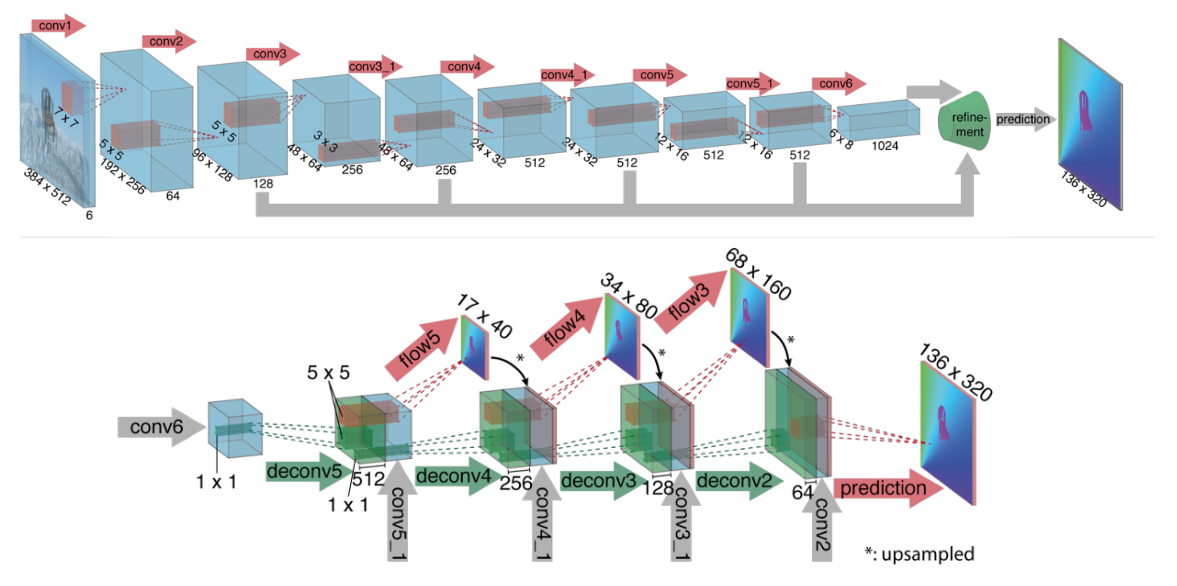
\includegraphics[scale=0.5]{figs/flow_net}
%    \end{adjustwidth}
%    \caption{
%        FlowNet architecture from \cite{FlowNet}.
%        At the top row the encoder is detailed, while the multi-scale decoder is shown at the bottom.
%        This architecture was first used for optical flow estimation and later adapted to depth estimation (starting from \cite{DispNet}).
%        \label{fig:flow_net}    
%    }
%\end{figure}
%As noted by Bhat~et~al~\cite{ZoeDepth}, larger backbones achieve better metrics.
%In recent years other architectures gained popularity, in particular transformer-based architectures~\cite{denseViT, PatchFusion} and diffusion models~\cite{Marigold}.
%Large Vision models (LVMs) are large neural networks trained on internet-scale data.
%Ke~et~al.~\cite{Marigold} adapted and fine-tuned an LVM based on diffusion to perform SIDE.
%The fine-tuning was performed on photo-realistic synthetic data and the resulting model showed zero-shot state of the art performances on various real world datasets.
%
%These works are opposed to the needs of robotics and autonomous driving.
%In such applications large neural networks present various problems.
%For instance, performing real-time inference on edge devices could be prohibitive.
%Most importantly, deep learning models are well known to be black-boxes.
%Their functioning is not understood by humans (it is said to be \textit{opaque}), this fact represents a problem in a critical application like driving.
%With the growing diffusion of neural network based software in society, its interaction with consumers and the need for regulatory laws, being able to understand and interpret these algorithms is a necessity.
%Explainable Artificial Intelligence (XAI) deals with this problem by developing methods for explaining deep learning models behavior~\cite{XAI_review}.
%Despite the popularity of XAI in the research community, only few works address the problem of explainability in SIDE~\cite{Hu, Dijk, towards_interpretable}.
%
%Objective of this thesis is to investigate the concept of interpretability, central to XAI, and its relation to SIDE.
%It is shown that some XAI research methods are biased and that there exist theoretical limitations to explainability that have consequences on this whole field of research.
%Such limitations stem from the inability of mathematical language to capture human related concepts like the one of "explanation", this fact is referred to as \textit{explanatory gap} (EG) throughout the thesis.
%It is argued that since SIDE involves aspects of human cognition, it is affected by the EG as well.
%Solving the SIDE task implies a minimum degree of opaqueness in the resulting method.
%This makes the use of non-interpretable components necessary for solving the depth estimation task.
%
%To reduce the impact of black-box methods on the overall interpretability of a SIDE pipeline, such methods must be confined to sub-tasks, leaving space for interpretable components.
%The responsibility of the final prediction is shared between non-interpretable and interpretable components.
%To further transfer responsibilities to the latter, the learning problem solved by the former has to be simplified.
%Toy experiments are then performed to test this approach applied to patch-wise depth estimation.
%The simplification of the learning problem is performed by carefully choosing the training patches, pre-processing them and using a different training loss and evaluation metrics. 
%Finally, an interpretable pipeline for merging partial depth estimates from the simplified learning problem is designed, but not tested.
%Results suggest that the practice of simplifying the learning problem can be beneficial since the model scores better metrics on the simplified learning problem.
%In future works, the ability of the interpretable pipeline to exploit partial predictions must be assessed.
%
%The rest of the thesis is organized as follows:
%\begin{itemize}
%    \item{
%        Chapter \ref{ch:sota} reviews various methods for SIDE.
%        Treated methods span from early days of the field to most recent developments.
%        The last two sections are about XAI and influential works on interpretability of SIDE models are presented.
%    }
%    \item{
%        Chapter \ref{ch:methods} addresses the problem of interpretability from a theoretical point of view.
%        The above claims about interpretability are supported in sections \ref{sec:limits of XAI}, \ref{sec:limits of interpretability} and \ref{sec:interpretability of depth estimation}.
%        In section \ref{sec:hybrid}, the formal theory of learning is quickly reviewed and possible simplifications to the problem of patch-wise depth estimation are presented and motivated.
%        The last section \ref{sec:depth_fusion} proposes a design for an interpretable algorithm that stitch together the partial patch predictions.
%    }
%    \item{
%        Chapter \ref{ch:results} presents and comments the experimental results obtained with the simplifications discussed in section \ref{sec:hybrid}.
%    }
%    \item{
%        Chapter \ref{ch:conc} closes this thesis by summing up its contributions and suggestions for future work.
%    }
%\end{itemize}